\documentclass[12pt%
%,draft%
,aspectratio=169%
]{beamer}
%
\usepackage{fontspec}
\defaultfontfeatures{Ligatures=TeX}
%\setsansfont{Liberation Sans}
\usepackage{polyglossia}
\setdefaultlanguage{ngerman}
% Alternative template for talks of the Freie Universität Berlin.
% Created by Leonard R. König, <leonard.koenig@fu-berlin.de> following the
% guidelines on www.fu-berlin.de/cd
%
% (c) Leonard König, CC BY 4.0
%
% This template was written against UTF-8 capable LaTeX engines, specifically
% LuaLaTeX.

% Trying to get rather close to the ppt/odp template:
%  http://www.fu-berlin.de/sites/cd/downloads_container/PowerPoint_Praesentation_Anleitung.pdf

%%% font styles
\setbeamerfont{frametitle}{series=\bfseries}
\setbeamerfont{footline}{series=\bfseries}
\setbeamerfont{headline}{series=\bfseries}
\setbeamerfont{alerted text}{series=\bfseries}
%%%

% colordefs
\definecolor{fu_darkblue}{RGB}{0,51,102}
\definecolor{fu_seablue}{RGB}{0,102,204}
\definecolor{fu_lightblue}{RGB}{204,214,224}
\definecolor{fu_green}{RGB}{153,204,0}
\definecolor{fu_lightgrey}{RGB}{128,128,128}
\definecolor{fu_grey}{RGB}{95,95,95}
%
\definecolor{fu_red}{RGB}{204, 0, 0} % red text (used by \alert)
%%% end colordefs

%%% colors
\setbeamercolor*{title}{fg=fu_darkblue}
\setbeamercolor*{subtitle}{fg=fu_seablue}
\setbeamercolor*{frametitle}{fg=fu_darkblue}
\setbeamercolor*{footline}{fg=fu_grey,bg=fu_lightblue}
\setbeamercolor*{headline}{fg=fu_grey}

\setbeamercolor*{normal text}{fg=black}
\setbeamercolor*{alerted text}{fg=fu_red}
\setbeamercolor*{example text}{fg=fu_green}
\setbeamercolor*{structure}{fg=fu_darkblue}

\setbeamercolor*{block title}{fg=white,bg=black!50}
\setbeamercolor*{block title alerted}{fg=white,bg=black!50}
\setbeamercolor*{block title example}{fg=white,bg=black!50}

\setbeamercolor*{block body}{bg=black!10}
\setbeamercolor*{block body alerted}{bg=black!10}
\setbeamercolor*{block body example}{bg=black!10}

\setbeamercolor{bibliography entry author}{fg=fu_darkblue}

\setbeamercolor{item}{fg=fu_darkblue}
\setbeamercolor{navigation symbols}{fg=fu_lightgrey,bg=fu_grey}
%%% end colors

%%% title page
% Display logo (if exists) and right next to it, put our title + subtitle
\defbeamertemplate*{title page}{fu_titlepage}
{%
	\hskip .3\textheight
	\begin{minipage}[.4\textheight]{\textwidth}
		\begin{minipage}[.4\textheight]{0.25\textwidth}
			\inserttitlegraphic
		\end{minipage}%
		\begin{minipage}[.4\textheight]{0.75\textwidth}
			\begin{beamercolorbox}{title}
				\usebeamerfont{title}\inserttitle\par%
			\end{beamercolorbox}
			\vfill
			\ifx\insertsubtitle
				\@empty%
			\else
				\begin{beamercolorbox}{subtitle}
					\usebeamerfont{subtitle}\insertsubtitle\par
				\end{beamercolorbox}
			\fi
		\end{minipage}
	\end{minipage}%
	\hskip .3\textheight
}
%%% end title page

%%% headline
% display title, author and institute on the left;
% logo on the right.
\newcommand{\headlinetext}
{%
	\inserttitle\\[0.3em]%
	\insertauthor, %
	\insertshortinstitute
}
\newlength{\headlinewidth}
\setlength{\headlinewidth}{\paperwidth}
\addtolength{\headlinewidth}{-2\marginparsep}
\setbeamertemplate{headline}
{%
	\begin{beamercolorbox}[wd=\paperwidth]{headline}%
		\vskip5pt
		{\hspace*{\marginparsep}}%
		\parbox{.5\headlinewidth}
		{%
			\usebeamertemplate{title in head/foot}%
			\headlinetext%
		}%
		\begin{minipage}{.5\headlinewidth}%
			\hfill\usebeamertemplate*{logo}
		\end{minipage}%
		{\hspace*{\marginparsep}}%
	\end{beamercolorbox}%
}
%%% end headline

%%% footline
% title + date on the left, frame number on the right
\newcommand{\footlinetext}
{%
	\usebeamerfont{shorttitle}\insertshorttitle, %
	\usebeamerfont{shortdate}\insertshortdate
}
\setbeamertemplate{footline}
{%
	\begin{beamercolorbox}{footline}
		\vskip2pt
		\hspace{\marginparsep}%
		\footlinetext\hfill%
		\insertframenumber%
		\hspace{\marginparsep}
		\vskip2pt
	\end{beamercolorbox}%
}
%%% end footline

% don't use default templates for sidebars
\setbeamertemplate{sidebar right}{}
\setbeamertemplate{sidebar left}{}
\setbeamertemplate{title page}[fu_titlepage]
\usepackage{amsmath}
\usepackage{amsfonts}
\usepackage{amssymb}
\usepackage{graphicx}
\usepackage{algorithm}
\usepackage[noend]{algpseudocode}
%\usepackage{algorithmic}
\usepackage{tikz}
\usetikzlibrary{arrows,shapes,automata,petri,positioning,calc}
\usepackage{graphicx}
\usepackage{subfig}
\usepackage{pgfplots}
\usepackage{venndiagram}



\pgfplotsset{
    standard/.style={%Axis format configuration
        axis x line=middle,
        axis y line=middle,
        enlarge x limits=0.15,
        enlarge y limits=0.15,
        every axis x label/.style={at={(current axis.right of origin)},anchor=north west},
        every axis y label/.style={at={(current axis.above origin)},anchor=north east},
        every axis plot post/.style={mark options={fill=white}}
        }
    }


\author{Benjamin Tröster}
\title[Bool'sche Algebra]{Bool'sche Algebra}
%\subtitle[Markov Models]{...}
%\pgfdeclareimage{titlegraphic}{../res/dwarf_logo2.png}
%\titlegraphic{\pgfuseimage{titlegraphic}}
%\date{}
%\subject{}
%
% FU settings
\institute[HTW Berlin]{Hochschule für Technik und Wirtschaft Berlin}
%\pgfdeclareimage[height=0.9cm]{logo}{../res/dwarf_logo}
%\logo{\pgfuseimage{logo}}
%
\usepackage[
backend=biber,
citestyle=alphabetic,bibstyle=authoryear
]{biblatex}
\addbibresource{sources.bib}


\begin{document}

\begin{frame}
\titlepage
\end{frame}

\begin{frame}{Fahrplan}
\tableofcontents[hideothersubsections]
\end{frame}

\section{Recap}
\subsection{Analoge/Digitale Signale}
\begin{frame}{Analoge/Digitale Signale}
\begin{definition}[Signal]
  		Informationstragende, physikalische Größe, die sich über der Zeit, über dem Ort oder über einer anderen Variablen ändert.
\end{definition}
\begin{itemize}
	\item Analoge Signale sind wert- \& zeitkontinuierlich
	\begin{itemize}
		\item Werte kontinuierlich (stetig)
		\item I.A. alle natürlichen physikalischen Signale \& Prozesse
	\end{itemize}
	\item Digitale Signale sind wert- \& zeitdiskret
	\begin{itemize}
		\item Diskrete Werte
		\item Variablen-Diskretisierung (Abtastung, führt zu diskreten Signalen)
		\item Amplituden- bzw. Wert-Diskretisierung (Quantisierung)
	\end{itemize}	
\end{itemize}
\end{frame}

\begin{frame}{Digital vs. Analog}
\begin{columns}[T] % align columns
\begin{column}{.48\textwidth}
\vspace{-1cm}
\begin{itemize}
		\item Analog:\\
		\begin{tikzpicture}[scale=.85]
  \begin{axis}%
    [grid=both,
     minor tick num=4,
     grid style={line width=.1pt, draw=gray!10},
     major grid style={line width=.2pt,draw=gray!50},
     axis lines=middle,
     enlargelimits={abs=0.2},
    ]
    \addplot[domain=-0:3,samples=50,smooth,red] {sin(deg(pi*x))};
  \end{axis}
\end{tikzpicture}
	\end{itemize} 
\end{column}%
\hfill%
\begin{column}{.48\textwidth}
\vspace{-1cm}
\begin{itemize}
	\item Digital:\\
\begin{tikzpicture}[scale=.85]
            \begin{axis}[%
            grid=both,
     minor tick num=4,
     grid style={line width=.1pt, draw=gray!10},
     major grid style={line width=.2pt,draw=gray!50},
     axis lines=middle,
     enlargelimits={abs=0.2},
                standard,
                domain = 0:3,
                samples = 32]
                \addplot+[ycomb,black,thick] {sin(deg(pi*x))};
            \end{axis}
        \end{tikzpicture}
        \end{itemize}
\end{column}%
\end{columns}
\end{frame}

\begin{frame}{Analog $\to$ Digital}
\vspace{-.74cm}
	\begin{figure}
	\centering
	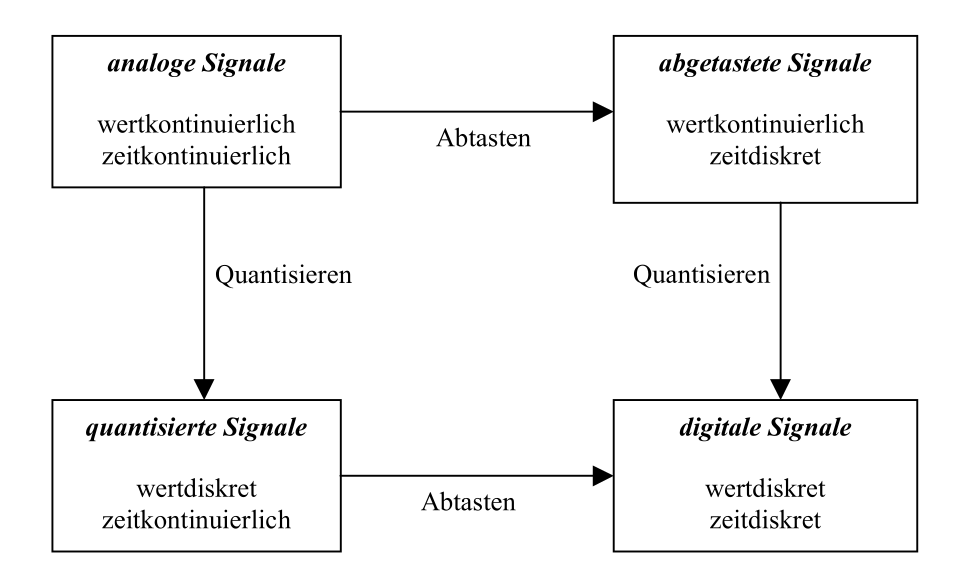
\includegraphics[scale=0.28]{pictures/adda}
	\end{figure}
\end{frame}

\begin{frame}{Grundlegende Signalverarbeitung: Deterministische Signale}
\begin{columns}[T] % align columns
\begin{column}{.6\textwidth}
\begin{itemize}
	\item Periodische Signale $\to$ deterministisch, Periode gibt fixen Bereich vor
	\item Parameter periodische Signale:
	\begin{itemize}
		\item Periode $T$
		\item Frequenz $f=\frac{1}{T}$, 
		\item Amplitude $S(t)$
		\item Phase $\varphi$
	\end{itemize}
	\item Beispiele:
	\begin{itemize}
		\item Sinus: Periode $2\pi$
		\item Phase shift $\varphi$ ($\sin \to \cos: \varphi= \frac{3}{2} \pi$)
	\end{itemize}
\end{itemize}
\end{column}%
\hfill%
\begin{column}{.4\textwidth}
\vspace*{-.75cm}
\begin{figure}
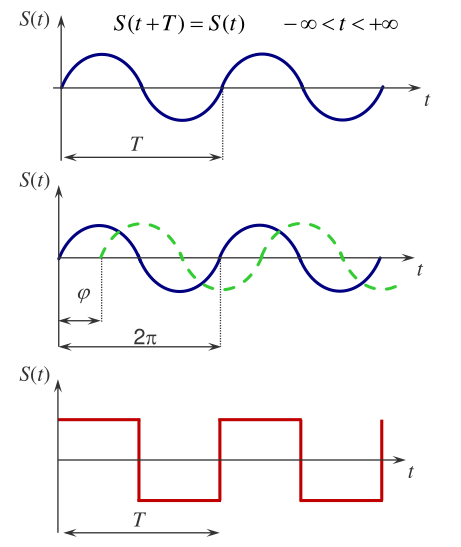
\includegraphics[scale=0.35]{pictures/sigproc}
\end{figure}
\end{column}%
\end{columns}
\end{frame}

\begin{frame}{Bit-Rate vs. Bandbreite: Signalfrequenz}
\begin{columns}[T] % align columns
\begin{column}{.6\textwidth}
\vspace*{-.7cm}
\begin{itemize}
	\item Ziel: Komposition der Rechteckschwingung durch periodische Funktion
	\item Signal besteht aus $f, 3f$ und $5f$
	\begin{itemize}
		\item $\sin(2\pi f t) + \frac{1}{3} sin(2 \pi 3 f t) + \frac{1}{5} sin(2 \pi 5 f t)$
	\end{itemize}
	\item Signal besteht aus $f, 3f, 5f$ und $7f$
	\begin{itemize}
		\item $\sin(2\pi f t) + \frac{1}{3} sin(2 \pi 3 f t) + \frac{1}{5} sin(2 \pi 5 f t) + \frac{1}{7} sin(2 \pi 7 f t)$
	\end{itemize}
	\item Rechteckschwingung:
	$$ s(t) = A \cdot \frac{4}{\pi} \cdot \sum_{k=1, k \text{ ungearde}}^\infty \frac{1}{k} \sin(2 \pi k f t) $$
\end{itemize}
\end{column}%
\hfill%
\begin{column}{.4\textwidth}
\vspace*{-.7cm}
\begin{figure}
\centering
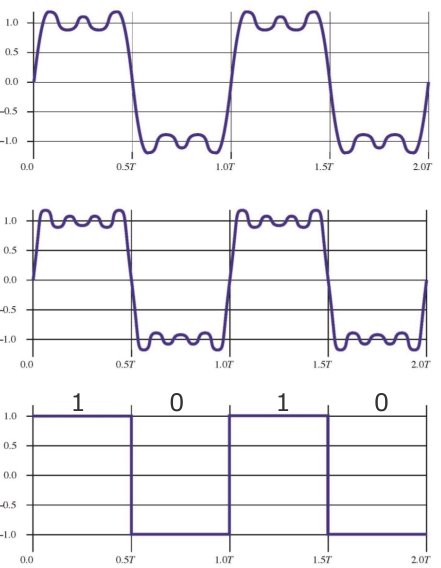
\includegraphics[scale=0.25]{pictures/sf}
\end{figure}
\end{column}%
\end{columns}
\end{frame}

\section{Einleitung}
\begin{frame}{Einleitung}
	\begin{itemize}
		\item Letzte Vorlesung: Wie kommen die Bits in den Rechner
		\item \textbf{Heute: Formale Beschreibung
			\begin{itemize}
				\item Logik, 
				\item Aussagenlogik 
				\item Bool'sche Algebra
\end{itemize}					
		}
		\begin{itemize}
			\item Formal: Was ist eine Aussage
			\item Aussagenlogik Axiomatisierung nach Peano/Huntington/Lattice
			\item Basisoperatoren, sekundäre Operatoren
		\end{itemize}
	\end{itemize}
\end{frame}

\subsection{Elementare Logik}
\begin{frame}{Elementare Logik}
\begin{definition}[Logik]
Eine \textbf{Aussage} (proposition) ist ein Satz, von dem man eindeutig entscheiden kann, ob er wahr oder falsch ist.
\end{definition}
\begin{itemize}
	\item Handelt es sich um eine Aussage?
	\begin{itemize}
		\item Wien ist die Hauptstadt von  Österreich.
		\item $1 + 5 = 6$.
		\item 5 ist kleiner als 3.
		\item Guten Abend!
		\item $x + 3 = 5$
	\end{itemize}
\end{itemize}
\cite{teschl2013mathematik}
\end{frame}

\subsection{Aussagenlogik}
\begin{frame}{Aussagenlogik}
\begin{definition}[Aussagenlogik]
\textbf{Aussagenlogik}, als Teilgebiet der Logik, befasst sich mit Aussagen und der Verknüpfung von Aussagen mittels \textit{Junktoren}.
\end{definition}
\begin{itemize}
	\item Junktoren sind logische Verknüpfungen
	\item Klassische Junktoren:
	\begin{itemize}
		\item Negation $\neg P$ 
		\item Implikation/Subjunktion/Konditional $P\Rightarrow Q$
		\item Äquivalenz/Bikonditional/Bisubjunktion $P\Leftrightarrow Q$
		\item Konjunktion $P\land Q$
		\item Disjunktion $P\lor Q$
	\end{itemize}
\end{itemize}
\cite{rautenberg2002einfuhrung}
\end{frame}

\begin{frame}{Negation}
\begin{definition}[Negation]
Sei $a$ beliebige Aussage, so ist die Verneinung oder Negation einer Aussage $a$ genau dann
wahr, wenn $a$ falsch ist. Die Verneinung von $a$ wird symbolisch mit $a$ oder $\neg a$ (auch $\overline{a}, !a$) bezeichnet (gelesen "nicht a").
\begin{center}
\begin{table}[]
\begin{tabular}{|c|c|ll}
\cline{1-2}
$a$ & $\neg a$ &  &  \\ \cline{1-2}
 0 & 1 &   \\ \cline{1-2}
 1 & 0 &   \\ \cline{1-2}
\end{tabular}
\end{table}
\end{center}
\end{definition}
\end{frame}

\begin{frame}{Implikation}
\begin{definition}[Aussagenlogik]
Seien $a$ und $b$ beliebige Aussagen, so ist die WENN-DANN-Verknüpfung oder Implikation $a \Rightarrow b$ (gelesen "Wenn a, dann b") wie folgt definiert:
\begin{center}
\begin{table}[]
\begin{tabular}{|c|c|c|ll}
\cline{1-3}
$a$ & $b$ & $a \Rightarrow b$ &  &  \\ \cline{1-3}
0 & 0 & 1 &  &  \\ \cline{1-3}
0 & 1 & 1 &  &  \\ \cline{1-3}
1 & 0 & 0 &  &  \\ \cline{1-3}
1 & 1 & 1 &  &  \\ \cline{1-3}
\end{tabular}
\end{table}
\end{center}
\end{definition}
\end{frame}


\begin{frame}{Äquivalenz}
\begin{definition}[Äquivalenz]
Seien $a$ und $b$ beliebige Aussagen, so ist die GENAU-DANN-Verknüpfung oder Bijunktion $a \Leftrightarrow b$ (gelesen "a genau dann, wenn b") von zwei Aussagen $a$ bzw. $b$ sind durch ihre Wahrheitstabellen folgendermaßen definiert:
\begin{center}
\begin{table}[]
\begin{tabular}{|c|c|c|ll}
\cline{1-3}
$a$ & $b$ & $a \Leftrightarrow b$ &  &  \\ \cline{1-3}
0 & 0 & 1 &  &  \\ \cline{1-3}
0 & 1 & 0 &  &  \\ \cline{1-3}
1 & 0 & 0 &  &  \\ \cline{1-3}
1 & 1 & 1 &  &  \\ \cline{1-3}
\end{tabular}
\end{table}
\end{center}
\end{definition}
\end{frame}


\begin{frame}{Konjunktion}
\begin{definition}[Konjunktion]
Seien $a$ und $b$ beliebige Aussagen, so ist die UND-Verknüpfung oder Konjunktion von $a$ und $b$ symbolisch mit $a \land b$ bezeichnet (gelesen: "a und b"). Die neue Aussage $a \land b$ ist genau dann
wahr, wenn sowohl $a$ als auch $b$ wahr ist. Ansonsten ist $a \land b$ falsch.
\begin{center}
\begin{table}[]
\begin{tabular}{|c|c|c|ll}
\cline{1-3}
$a$ & $b$ & $a \land b$ &  &  \\ \cline{1-3}
0 & 0 & 0 &  &  \\ \cline{1-3}
0 & 1 & 0 &  &  \\ \cline{1-3}
1 & 0 & 0 &  &  \\ \cline{1-3}
1 & 1 & 1 &  &  \\ \cline{1-3}
\end{tabular}
\end{table}
\end{center}
\end{definition}
\end{frame}

\begin{frame}{Return to Äquivalenz}
Die Äquivalenz kann auch als Kombination zweier Implikationen betrachtet werden:\\
$$a \Rightarrow b \land a \Leftarrow b$$
\end{frame}

\begin{frame}{Return to Äquivalenz}
Die Äquivalenz kann auch als Kombination zweier Implikationen betrachtet werden:\\
$a \Rightarrow b \land a \Leftarrow b$
\begin{center}
\begin{table}[]
\begin{tabular}{|c|c|c|ll}
\cline{1-3}
$a$ & $b$ & $a \Rightarrow b$ &  &  \\ \cline{1-3}
0 & 0 & 1 &  &  \\ \cline{1-3}
0 & 1 & 1 &  &  \\ \cline{1-3}
1 & 0 & 0 &  &  \\ \cline{1-3}
1 & 1 & 1 &  &  \\ \cline{1-3}
\end{tabular}
%
\begin{tabular}{|c|c|c|ll}
\cline{1-3}
$b$ & $a$ & $b \Rightarrow a$ &  &  \\ \cline{1-3}
0 & 0 & 1 &  &  \\ \cline{1-3}
0 & 1 & 1 &  &  \\ \cline{1-3}
1 & 0 & 0 &  &  \\ \cline{1-3}
1 & 1 & 1 &  &  \\ \cline{1-3}
\end{tabular}
%
\begin{tabular}{|c|c|c|ll}
\cline{1-3}
$A: a \Rightarrow b$ & $B: a \Leftarrow b$ & $A \land B$ &  &  \\ \cline{1-3}
0,0 $\to$ 1 & 0,0 $\to$ 1 & 1 &  &  \\ \cline{1-3}
0,1 $\to$ 1 & 1,0 $\to$ 0 & 0 &  &  \\ \cline{1-3}
1,0 $\to$ 0 & 1,0 $\to$ 0 & 0 &  &  \\ \cline{1-3}
1,1 $\to$ 1 & 1,1 $\to$ 1 & 1 &  &  \\ \cline{1-3}
\end{tabular}
\end{table}

\end{center}

\end{frame}

\begin{frame}{Disjunktion}
\begin{definition}[Disjunktion]
Seien $a$ und $b$ beliebige Aussagen, so ist ODER-Verknüpfung oder Disjunktion von $a$ und $b$ symbolisch mit $a \lor b$ bezeichnet (gelesen: "a oder b"). Die neue Aussage $a \lor b$ ist genau dann wahr, wenn mindestens eine der beiden Aussagen $a$ bzw. $b$ wahr ist; sonst ist $a \lor b$ falsch. Die Verknüpfung $a \lor b$ entspricht dem nicht-ausschließenden "oder" der Umgangssprache (denn $a \lor b$ ist auch wahr, wenn sowohl $a$ als auch $b$ wahr ist)!
\begin{center}
\begin{table}[]
\begin{tabular}{|c|c|c|ll}
\cline{1-3}
$a$ & $b$ & $a \lor b$ &  &  \\ \cline{1-3}
0 & 0 & 0 &  &  \\ \cline{1-3}
0 & 1 & 1 &  &  \\ \cline{1-3}
1 & 0 & 1 &  &  \\ \cline{1-3}
1 & 1 & 1 &  &  \\ \cline{1-3}
\end{tabular}
\end{table}
\end{center}
\end{definition}

\end{frame}

\section{Bool'sche Algebra}

\begin{frame}{Algebra}
\begin{definition}[Algebra]
Als Teilgebiete der Mathematik befasst sich die Algebra mit den Eigenschaften von Rechenoperationen.
\end{definition} 
Verkürzt aus \cite{bewersdorff2007algebra}
\end{frame}


\begin{frame}{Bool'sche Algebra}
\begin{definition}[BA nach Peano]
Die bool'sche Algebra nach Peano ist als Menge $\mathcal{V}$ mit Nullelement $0$ und Einselement $1$ und den zweistelligen Verknüpfungen $\land (\cdot)$, $\lor (+)$, sowie der einstelligen Verknüpfung $\neg$ definiert.
\end{definition}
\begin{itemize}
	\item Definitionsmenge $\mathcal{D}: \{0,1\}^*$, Zielmenge $\mathcal{Z}: \{0,1\}$
	\item Einstellige Verknüpfung: $f: \{0,1\} \to \{0,1\}$
	\item Zweistellige Verknüpfung: $f: \{0,1\} \times \{0,1\} \to \{0,1\}$
	\item $n$-stelligen Verknüpfung $f : \{0, 1\}^n \to \{0, 1\}$
	\item Gesamtheit wird mit $B_n$ bezeichnet, daraus ergeben sich $2^n$ Funktionen
	\item $B_0$ sind die Konstanten $0$ und $1$
\end{itemize}
\end{frame}


\begin{frame}{Bool'sche Algebra nach Peano}
\begin{enumerate}
	\item Kommutativgesetz (K) $a \land b = b \land a$ bzw. $a \lor b = b \lor a$
	\item Assoziativgesetz (A) $(a \land b ) \land c = a \land ( b \land c )$ bzw. $(a \lor b ) \lor c = a \lor ( b \lor c )$
	\item Idempotenzgesetz (I) $a \land a = a$ bzw. $a \lor a = a$
	\item Distributivgesetz (D) $a \land ( b \lor c ) = ( a \land b ) \lor ( a \land c )$ bzw. $a \lor ( b \land c ) = ( a \lor b ) \land ( a \lor c ) $
	\item Neutralitätsgesetz (N) $a \land 1 = a$ bzw. $a \lor 0 = a$
	\item Extremalgesetz (Ex) $a\land 0=0$ bzw. $ a\lor 1=1$
	\item Involution (In) $\neg(\neg a)=a $
	\item De Morgansche Gesetz $\neg(a \land b)=\neg a \lor \neg b$ bzw. $\neg(a\lor b)=\neg a\land\neg b$
	\item Komplementärgesetz/Inverse Element (I) $a\land\neg a=0$ bzw. $a\lor\neg a=1$
	\item Dualitätsgesetz 	$\neg 0 = 1$ bzw. $\neg 1 = 0$
	\item Absorptionsgesetz $a\lor(a\land b)=a$ bwz. $a\land (a\lor b)=a$
\end{enumerate}
\end{frame}

\begin{frame}{Bool'sche Algebra nach Huntington (\textbf{Wichtig!})}
\begin{definition}
Die bool'sche Algebra nach Huntington ist definiert als Menge $\mathcal{V}: \{0,1\}$ mit den Verknüpfungen $\cdot (\land), + (\lor)$, sodass $\mathcal{V} \times \mathcal{V} \to \mathcal{V}$, also $\{0,1\} \times \{0,1\} \to \{0,1\}$. 
\end{definition}
\begin{itemize}
	\item Kommutativgesetze (K): $a \cdot b = b \cdot a$ bzw. $a + b = b + a$
	\item Distributivgesetze (D): $a \cdot (b + c) = (a \cdot b) + (a \cdot c)$ bzw. $a + (b \cdot c) = (a + b) \cdot (a + c)$
	\item Neutrale Elemente (N): $ \exists e, n \in \mathcal{V}$ mit  $a \cdot e = a$ und $a + n = a$
	\item Inverse Elemente (I): $\forall a \in \mathcal{V}$ existiert ein $a'$ mit $a \cdot a'= n$ und $a + a' = e$
\end{itemize}
Übernommen von \cite{barnett2013boolean} bzw. \cite{hoffmann2020grundlagen}
\end{frame}

\begin{frame}{Bool'sche Algebra als Verband (Lattice)}
\begin{definition}
Es kann eine bool'sche Algebra mit den Verknüpfungen $\land, \lor, \neg$ und den Elementen $0,1$ als distributiver, komplementärer Verband definiert werden. Zusätzlich ist eine partielle Halbordnung $a \leq b \Leftarrow a = a \land b$ definiert. So haben zwei Elemente ein Supremum und ein Infimum.
\end{definition}
\begin{itemize}
	\item Kommutativgesetze (K): $a \land b = b \land a$ bzw. $a \lor b = b \lor a$
	\item Assoziativgesetz (A) $(a \land b ) \land c = a \land ( b \land c )$ bzw. $(a \lor b ) \lor c = a \lor ( b \lor c )$
	\item Absorptionsgesetz $a\lor(a\land b)=a$ bwz. $a\land (a\lor b)=a$
	\item Komplementärgesetz/Inverse Element (I) $a\land\neg a=0$ bzw. $a\lor\neg a=1$
	\item Distributivgesetz (D) $a \land ( b \lor c ) = ( a \land b ) \lor ( a \land c )$
\end{itemize}
\cite{sasao1999lattice}
\end{frame}

\subsection{Darstellungen}
\begin{frame}{Darstellungen}
\begin{itemize}
	\item Wahrheitstabelle (s.o.)
	\item Via Graph $y = ((0 \land x) ∨ (1 \lor x))$\\
	\resizebox{5cm}{!}{%
\begin{tikzpicture}[>=stealth',auto,shorten >=1pt]
    \node [place] (tlor) {$\lor$};
    
    \node [place] (llor) [below left=of tlor] {$\land$};
	\node [place] (rlor) [below right=of tlor] {$\land$};
	\node [place] (b0) [below left=of llor] {$0$};
	\node [place] (bx) [below =of llor] {$x$};
	
	\node [place] (b1) [below =of rlor] {$1$};
	\node [place] (bx2) [below right=of rlor] {$x$};

	\path[-] (tlor) edge node [left] {}  (llor);
	\path[-] (tlor) edge node [left] {}  (rlor);
	\path[-] (llor) edge node [left] {}  (b0);
	\path[-] (llor) edge node [left] {}  (bx);
	\path[-] (rlor) edge node [left] {}  (b1);
	\path[-] (rlor) edge node [left] {}  (bx2);

\end{tikzpicture}
}
	\item Formeldarstellung -- algebraische Darstellung (s.o)
\end{itemize}
\end{frame}

\section{Schaltalgebra}
\begin{frame}{Schaltalgebra als bool'sche Algebra}
\begin{itemize}
	\item $\neg, \land$ und $\lor$ sind Operatoren über der Menge $\{0,1\}$
\begin{center}

\begin{table}[]
\begin{tabular}{|c|c|c|ll}
\cline{1-3}
$a$ & $b$ & $a \land b$ &  &  \\ \cline{1-3}
0 & 0 & 0 &  &  \\ \cline{1-3}
0 & 1 & 0 &  &  \\ \cline{1-3}
1 & 0 & 0 &  &  \\ \cline{1-3}
1 & 1 & 1 &  &  \\ \cline{1-3}
\end{tabular}
%
\begin{tabular}{|c|c|c|ll}
\cline{1-3}
$a$ & $b$ & $a \lor b$ &  &  \\ \cline{1-3}
0 & 0 & 0 &  &  \\ \cline{1-3}
0 & 1 & 1 &  &  \\ \cline{1-3}
1 & 0 & 1 &  &  \\ \cline{1-3}
1 & 1 & 1 &  &  \\ \cline{1-3}
\end{tabular}
%
\begin{tabular}{|c|c|ll}
\cline{1-2}
$a$ & $\neg a$ &  &  \\ \cline{1-2}
 0 & 1 &   \\ \cline{1-2}
 1 & 0 &   \\ \cline{1-2}
\end{tabular}
\end{table}
\end{center}
	\item Kommutativgesetze, Distributivgesetze, neutrales Element, inverses Element
	\begin{table}[]
	\begin{tabular}{ccc}
$\mathcal{V}$ & $\{0,1\}$ & Wahrheitswerte (TRUE, FALSE) \\
	$\cdot$ & $\land$ & Konjunktion (UND-Operator) \\
	$+$ & $\lor$ & Disjunktion (ODER-Operator) \\
	$n$ & $0$ & Falsch (FALSE)\\
	$e$ & $1$ &  Wahr (TRUE)\\
	$a'$ & $\neg a$ & Negation (Verneinung)\\
\end{tabular}
\end{table}
\end{itemize}
\end{frame}

\section{Mengenalgebra}
\begin{frame}{Mengenalgebra}
	\begin{definition}[Trägermenge]
	 Eine Trägermenge $\mathcal{T}$ bezeichnet die Menge, die mithilfe einer Menge von Verknüpfungen eine algebraische Struktur bildet.
	\end{definition}
\begin{itemize}
	\item Mengenalgebra über einer Trägermenge $\mathcal{T}$ 
\begin{center}
	\begin{table}[]
	\begin{tabular}{ccc}
$\mathcal{V}$ & $\mathcal{P}(T)$ & Potenzmenge der Trägermenge T \\
	$\cdot$ & $\cap$ & Durchschnitt \\
	$+$ & $\cup$ & Leere Menge \\
	$n$ & $\emptyset$ & Falsch (FALSE)\\
	$e$ & $\mathcal{T}$ &  Trägermenge\\
	$a'$ & $\mathcal{T} \setminus A$ & Komplementärmenge\\
\end{tabular}
\end{table}
\end{center}
\end{itemize}
\end{frame}

\begin{frame}{Mengenalgebra}

	\begin{center}
\begin{venndiagram2sets}
       \fillNotA
\end{venndiagram2sets}
\begin{venndiagram2sets}
       \fillA \fillB
\end{venndiagram2sets}
\begin{venndiagram2sets}
       \fillACapB
\end{venndiagram2sets}
\end{center}
\end{frame}

\section{Notation und Operatorenbindung}
\begin{frame}{Notation und Operatorenbindung}
\begin{itemize}
	\item Syntactic Sugar (Ableitungen aus Basisverknüpfungen)
	\begin{itemize}
		\item $(a \Rightarrow b)$ für $(\neg a \lor b)$ -- Implikation
		\item $(a \Leftarrow b)$ für $(b \Rightarrow a)$ -- Inversion der Implikation
		\item $(a \Leftrightarrow b)$ für $(a \Rightarrow b) \land (a \Leftarrow b)$ -- Äquivalenz
		\item $(a \oplus b)  für ¬(a \Leftrightarrow b$ -- Antivalenz oder Exklusiv-ODER/XOR
		\item $\neg(a \lor b)$ -- NOR
		\item $\neg (a \land b)$ -- NAND
	\end{itemize}
	\item Bindung der Operatoren 
	\begin{itemize}
		\item $\land$ bindet stärker als $\lor$
		\item $\neg$ bindet stärker als $\land$
	\end{itemize}
	\item Klammerung
	\begin{itemize}
		\item Gleiche Verknüpfungen: linksassoziativ zusammengefasst
	\end{itemize}
\end{itemize}	 
\end{frame}

\begin{frame}{Weitere Verknüpfungen}
\begin{figure}
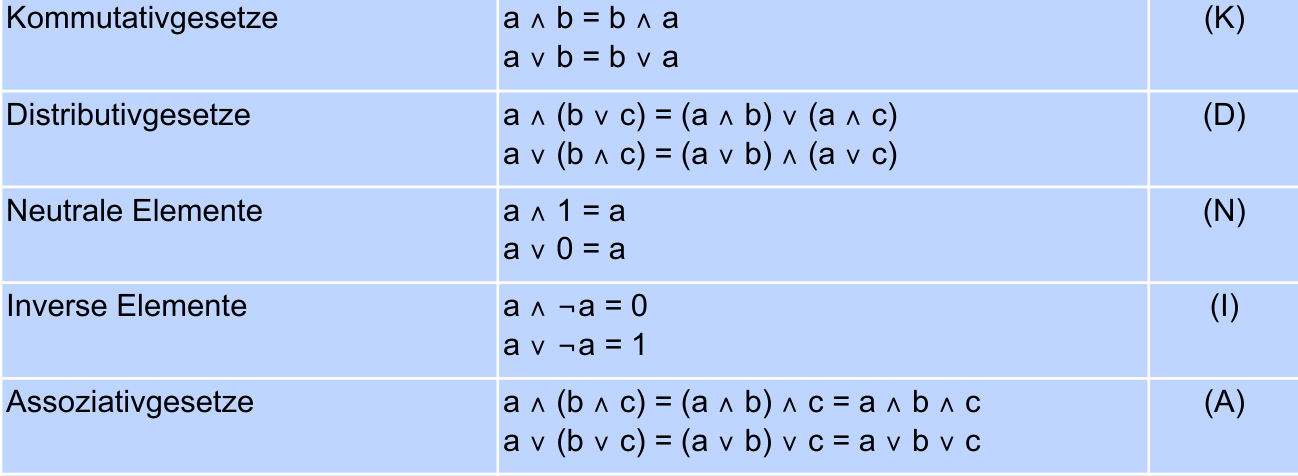
\includegraphics[scale=0.325]{pictures/ops1.png}
\end{figure}
\cite{hoffmann2020grundlagen}
\end{frame}

\begin{frame}{Weitere Verknüpfungen}
\begin{figure}
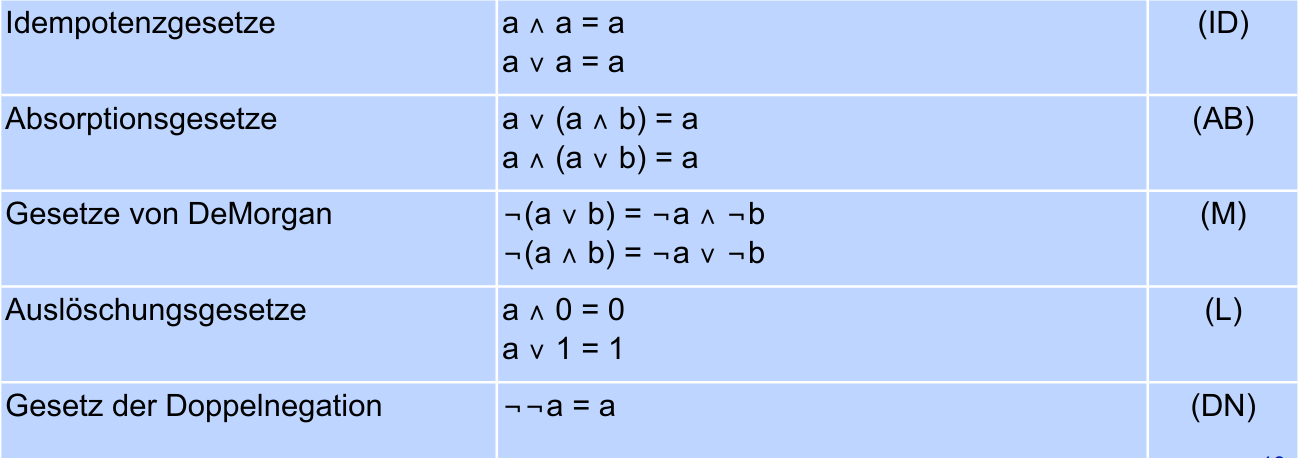
\includegraphics[scale=0.325]{pictures/ops2}
\end{figure}
\cite{hoffmann2020grundlagen}
\end{frame}

\begin{frame}{Beispiel}
$$ Y = (A \lor B) \land (\neg A \lor B) \land (A \lor \neg B) $$
\end{frame}

\section{Ausblick}
\begin{frame}{Ausblick nächste Vorlesung}
\begin{itemize}
	\item Universelle Operatoren
	\item De Morgan Regeln
	\item Normalformen
	\item Beweisstrategien \& Induktion
	\item Bitweise logische Operationen, Bit-Maskierung
	\item Einführung Logikgatter
\end{itemize}

\end{frame}

\section*{Quellen}
\appendix
\begin{frame}[allowframebreaks]
  \frametitle<presentation>{Quellen}
\printbibliography
\end{frame}
\end{document}